\documentclass[11pt]{article}
\usepackage[margin=1in]{geometry}
\usepackage{amsmath}
\usepackage{graphicx}
\usepackage{hyperref}
\usepackage{float}

\title{Exoplanet Parameter Estimation Showcase\\\large Reconstructing and Modernizing a Legacy Prototype}
\author{Mauricio Tedeschi}
\date{\today}

\begin{document}
\maketitle

\begin{abstract}
This document accompanies the rebuilt \texttt{exoplanet-parameter-estimation-model}
project. The recovered archive contained a three-script prototype, four
real Doppler time-series CSVs, a stellar mass table, and two draw.io design
artifacts. The rebuild packages that work into a reproducible \texttt{uv}-managed
Python project with a Keplerian radial-velocity model, differential-evolution
search, local least-squares refinement, synthetic validation, and physics-based
orbit visualization. This report summarizes the archived workflow, explains the
updated modeling pipeline, and documents results on both synthetic data and the
recovered \texttt{star0} observation set.
\end{abstract}

\section{Archived Material}

The recovered archive contributed the following assets:
\begin{itemize}
    \item legacy scripts: \texttt{graphcomparison.py}, \texttt{nbodysolver.py}, and \texttt{rvdatareader.py}
    \item a stellar mass catalog for four systems
    \item four real Doppler-shift datasets: \texttt{star0.csv} through \texttt{star3.csv}
    \item two draw.io diagram files labeled ``M\_p and R space'' and ``M\_p and R space after iteration''
\end{itemize}

The archive did not include a finished paper or \LaTeX{} manuscript, so this
report serves as a reconstructed write-up grounded in the recovered code,
datasets, and the new implementation.

\section{Legacy Prototype}

The original project estimated exoplanet parameters by combining three pieces:
\begin{enumerate}
    \item Doppler-shift CSV ingestion
    \item a two-body Euler integrator for star--planet motion
    \item a geometric-mean search over planet mass and orbital radius
\end{enumerate}

That approach had educational value and preserved the physical intuition of a
star wobbling around the system barycenter. However, it also mixed the expensive
numerical integrator directly into the fitting loop, depended on missing local
CSV files, and was difficult to reproduce or extend.

\section{Modernized Pipeline}

The rebuild keeps the same scientific story while separating \emph{modeling},
\emph{optimization}, and \emph{visualization}.

\subsection{Doppler Conversion}

The archived files store Doppler shift $z$ instead of radial velocity $v$. The
package converts between the two using the relativistic relation
\begin{equation}
z = \sqrt{\frac{1 + \beta}{1 - \beta}} - 1,
\qquad
\beta = \frac{v}{c},
\end{equation}
which can be inverted to recover stellar radial velocity from each observed
shift value.

\subsection{Keplerian Radial-Velocity Model}

For fitting, the rebuilt code uses an analytic single-planet Keplerian model:
\begin{equation}
v_r(t) = \gamma + K \left[\cos(\omega + \nu(t)) + e \cos(\omega)\right],
\end{equation}
where $K$ is the radial-velocity semi-amplitude, $P$ is the orbital period,
$e$ is eccentricity, $\omega$ is the argument of periastron, $t_0$ is the
periastron time, and $\gamma$ is the system velocity offset. The true anomaly
$\nu(t)$ is recovered by solving Kepler's equation for the eccentric anomaly and
then transforming into orbital phase.

\subsection{Optimization Strategy}

Instead of evaluating a numerical integrator at every candidate point, the new
pipeline:
\begin{enumerate}
    \item performs a global search with \texttt{scipy.optimize.differential\_evolution}
    \item refines the best candidate with \texttt{scipy.optimize.least\_squares}
    \item derives a representative planet mass and semi-major axis from the fitted
    semi-amplitude and stellar mass under an edge-on assumption
\end{enumerate}

This split makes fitting fast enough to run as a repeatable example while still
preserving a physically interpretable orbit plot.

\subsection{Orbit Visualization}

After fitting, the project constructs barycentric initial conditions and
integrates a two-body orbit using the velocity Verlet method. The resulting
orbit panel is not used for optimization; it is a clean post-fit visualization
that keeps the original project's dynamical flavor without the numerical drift
of the Euler loop.

\section{Datasets}

\subsection{Synthetic Validation}

The repository now ships a synthetic-data generator. A reference system with
known $K$, $P$, $e$, stellar mass, and planet mass is sampled at irregular
observation times, corrupted with measurement noise, and then passed through the
same fitting pipeline. This gives a reproducible benchmark for validating the
rebuild.

\subsection{Recovered Observation Data}

The archived real observations are now versioned under
\texttt{data/archived\_observations/}. The stellar mass catalog is:
\begin{center}
\begin{tabular}{l l}
\texttt{star0}: 1.11 $M_{\odot}$ & \texttt{star2}: 2.30 $M_{\odot}$ \\
\texttt{star1}: 1.39 $M_{\odot}$ & \texttt{star3}: 1.34 $M_{\odot}$ \\
\end{tabular}
\end{center}

The rebuilt example script currently demonstrates \texttt{star0}, matching the
legacy prototype's original short test case and providing a compact real-data
sanity check for the new package.

\section{Results}

\subsection{Synthetic Benchmark}

For the synthetic showcase system, the recovered fit is close to the planted
truth:
\begin{itemize}
    \item truth: $P = 147.5$ days, $K = 30.5$ m/s, $M_p = 0.82~M_J$, $e = 0.19$
    \item recovered: $P = 147.16$ days, $K = 31.35$ m/s, $M_p = 0.836~M_J$, $e = 0.221$
    \item residual RMS: 2.11 m/s
\end{itemize}

\begin{figure}[H]
    \centering
    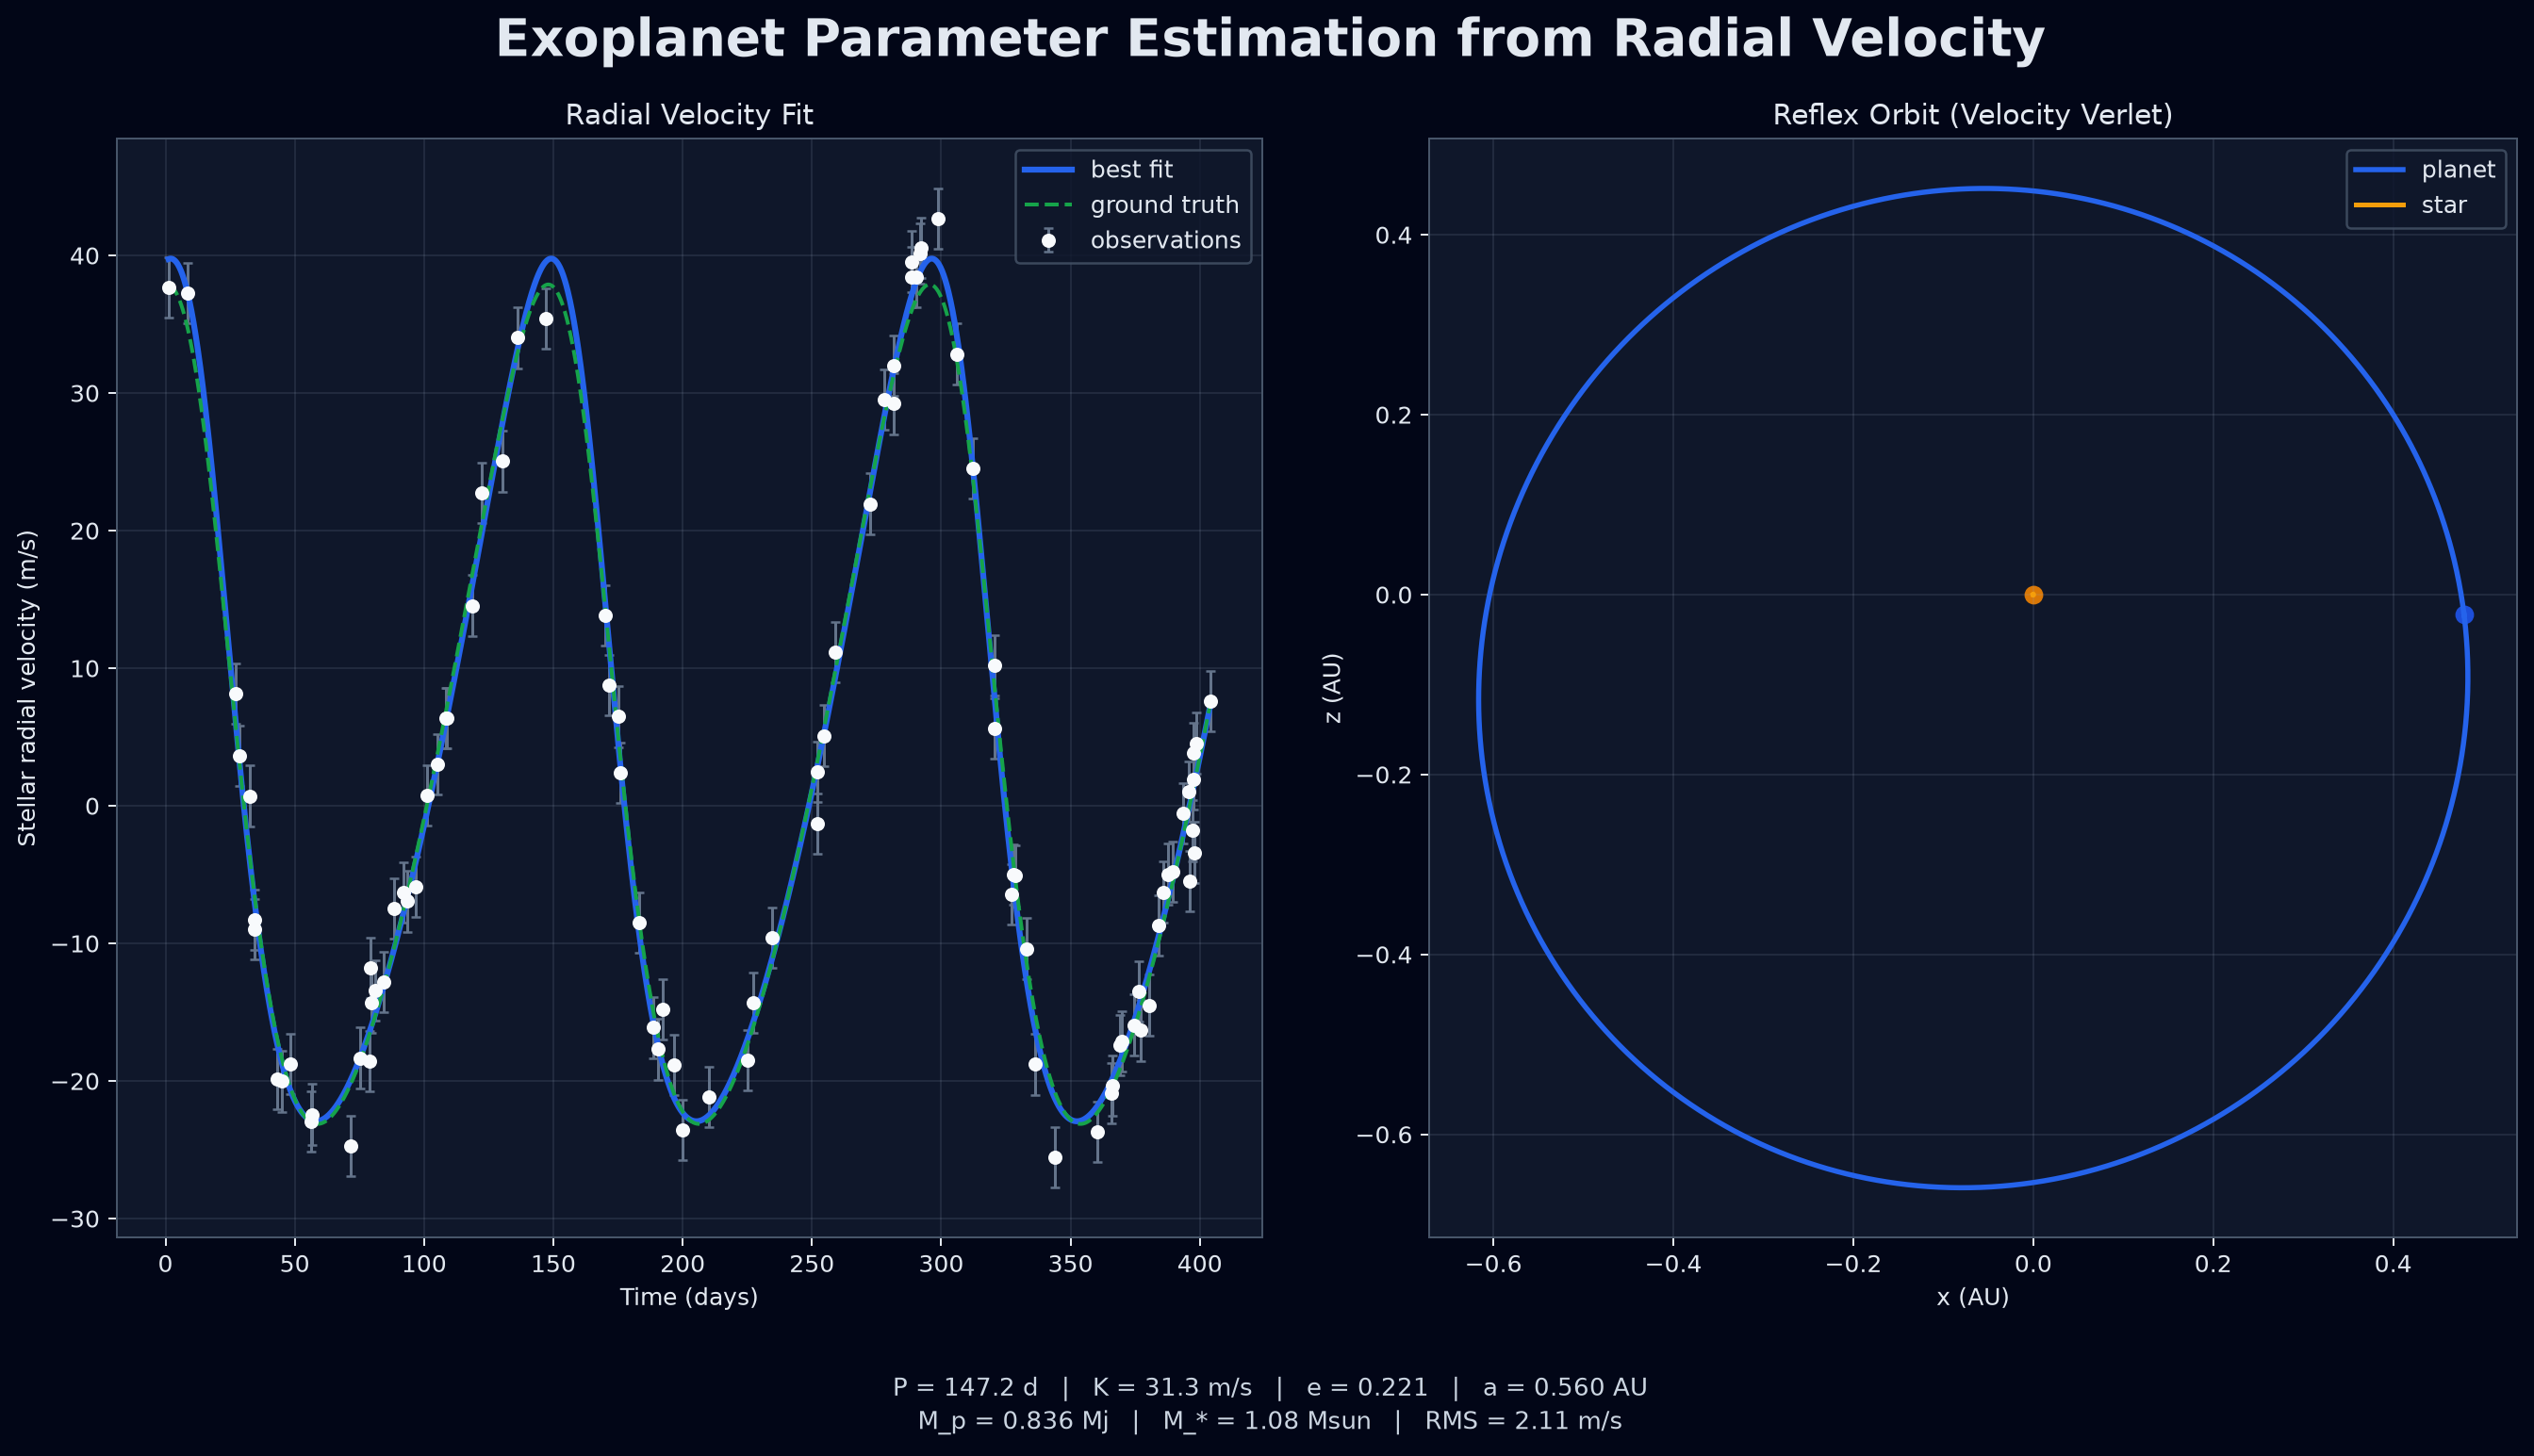
\includegraphics[width=\textwidth]{figures/rv_fit_preview.png}
    \caption{Synthetic validation example included in the rebuilt repository. The
    left panel shows noisy radial-velocity samples with the recovered Keplerian fit;
    the right panel shows the corresponding barycentric orbit rendered with the
    velocity Verlet integrator.}
\end{figure}

\subsection{Recovered \texttt{star0} Fit}

Running the new real-data example on \texttt{star0} yields:
\begin{itemize}
    \item stellar mass: $1.11~M_{\odot}$
    \item fitted period: 4.269 days
    \item fitted semi-amplitude: 56.694 m/s
    \item fitted eccentricity: 0.002
    \item derived planet mass: $0.485~M_J$
    \item residual RMS: 5.23 m/s
\end{itemize}

\begin{figure}[H]
    \centering
    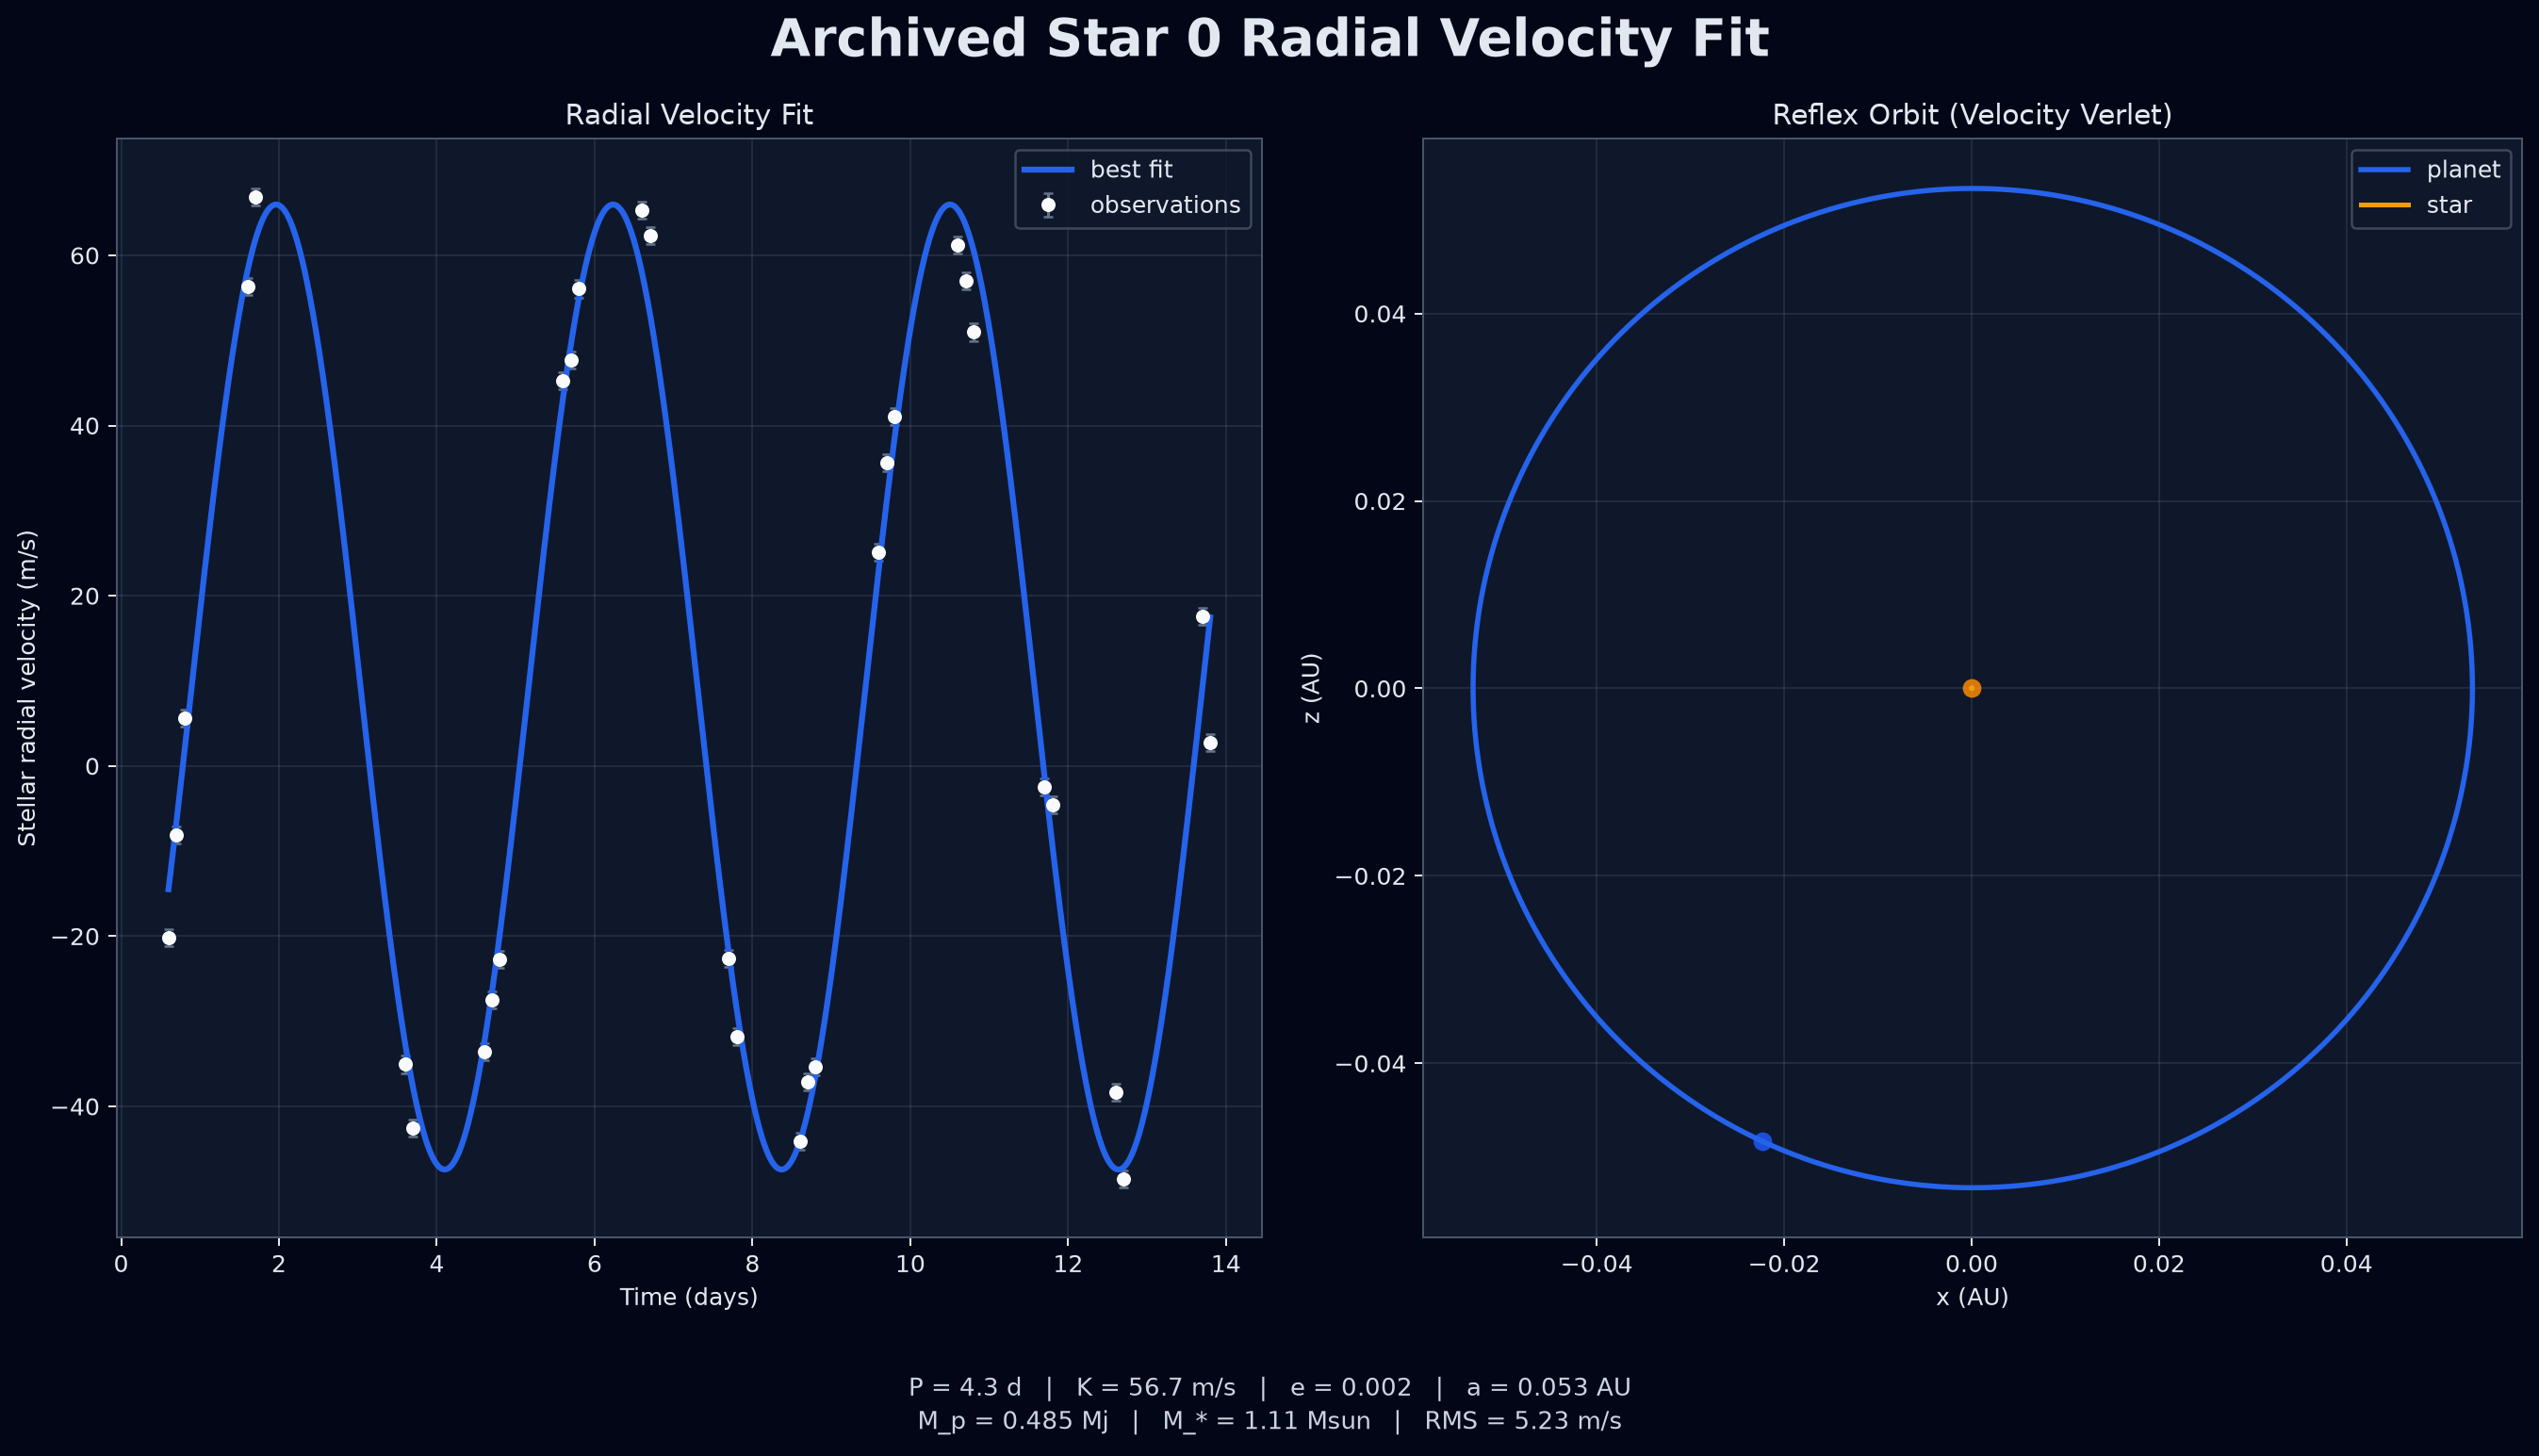
\includegraphics[width=\textwidth]{figures/archived_star0_fit.png}
    \caption{Recovered fit for the archived \texttt{star0} dataset. The nearly
    circular best fit and short orbital period make this a clean real-data example
    for the rebuilt package.}
\end{figure}

\section{Repository Additions}

The rewrite now includes:
\begin{itemize}
    \item packaged source code under \texttt{src/exoplanet\_est/}
    \item synthetic and real-data example scripts
    \item archived CSVs under \texttt{data/archived\_observations/}
    \item documentation figures under \texttt{docs/figures/}
    \item this \LaTeX{} report as a companion artifact
\end{itemize}

\section{Limitations and Next Steps}

The current package intentionally focuses on the clean single-planet case. A few
natural extensions would be:
\begin{itemize}
    \item support explicit measurement uncertainties and instrument offsets when
    available
    \item add periodogram-based initialization for the longest archival datasets
    \item extend the model to multiple planets or Bayesian posterior estimation
    \item convert the draw.io design artifacts into polished report figures if a
    future revision needs more visual explanation of the original search space
\end{itemize}

\section{Reproduction}

The core commands are:
\begin{verbatim}
uv sync
MPLBACKEND=Agg uv run python examples/fit_synthetic.py --save outputs/rv_fit_preview.png
MPLBACKEND=Agg uv run python examples/fit_archived_star.py --star-index 0 \
  --save outputs/archived_star0_fit.png
latexmk -pdf -cd docs/exoplanet_showcase_report.tex
\end{verbatim}

\noindent
Together, these commands reproduce the synthetic benchmark, the archived
\texttt{star0} fit, and the compiled report.

\end{document}
